\documentclass[a4paper,12pt,leqno,titlepage]{article}
\usepackage{hyperref} %linkitys
\usepackage[titletoc]{appendix}
\usepackage{graphicx}
\usepackage{listings}
\usepackage{moreverb}
\usepackage{amsmath}
\usepackage{amsthm}
\usepackage[finnish]{babel}
\usepackage{ucs}
\usepackage[utf8x]{inputenc}
\usepackage{amssymb}
%\usepackage{harvard}
%\usepackage{authordate1-4}
\usepackage[sorting=none]{biblatex}
\usepackage{pgfplots}
%\pgfplotsset{width=7cm}%,compact=1.10}

\widowpenalty=1000
\clubpenalty=1000

\setlength{\parskip}{2ex plus 2ex minus 1ex}

%\usepackage[comma,authoryear,numbers]{natbib}
\newcommand{\R}{\mathbb{R}} %lukujoukkosymbolit
\newcommand{\C}{\mathbb{C}}
\newcommand{\Q}{\mathbb{Q}}
\newcommand{\N}{\mathbb{N}}
\newcommand{\Z}{\mathbb{Z}}
\newcommand{\logM}{\mathcal{M}}
\setlength{\parindent}{0pt} %kappalejakoa
%\setlength{\parskip}{2ex}
\newcommand{\compcent}[1]{\vcenter{\hbox{$#1\circ$}}}
\newcommand{\comp}{\mathbin{\mathchoice
{\compcent\scriptstyle}{\compcent\scriptstyle}
{\compcent\scriptscriptstyle}{\compcent\scriptscriptstyle}}}

%\hyphenpenalty=750
%\setlength{\emergencystretch}{1.5 em} % Tavutusasetukset suomen kielelle

\hypersetup{
pdfborder = {0 0 0 0}, %linkkien värejä etc kikkailua
colorlinks = true,
linkcolor = black,
urlcolor = blue,
citecolor = red,
}


\usepackage{lastpage} %sivumäärä alaviitteeseen
\usepackage{fancyhdr}

\pagestyle{fancy}
\cfoot{Sivu \thepage/\pageref{LastPage}}

\bibliography{tutkimussuunnitelma}{}

\begin{document}
\begin{titlepage}
\title{Miten oppilaat kokevat laskupajamuotoisen työskentelyn?} %Laskupajamuotoinen opetus lukiotasolla}
\author{Sandra Luhtaniemi ja Aleksi Markkanen\\
Opiskelijanumerot 013734363 ja 013126382\\
\pageref{LastPage} sivua}
\date{\today}
\end{titlepage}
\maketitle
\pagebreak
\tableofcontents
\pagebreak

\section{Johdanto}
Kisälliopetus on uusi ja innovatiivinen tapa opettaa matematiikkaa. Aihe on ajankohtainen, sillä sen tiimoilta on tehty lähivuosina tutkimusta Helsingin yliopistossa sekä matematiikan- ja tilastotieteen laitoksella että tietojenkäsittelytieteen laitoksella.
Se eroaa merkittävästi perinteisestä matematiikan opetuksesta, jossa uusi asia luennoidaan ja kotiläksyksi annetaan tehtäviä, jotka liittyvät tunnilla käytyihin asioihin.
Kisälliopetuksessa korostetaan laskemisen ja tekemällä oppimisen merkitystä. Opiskelijan ajatellaan sisäistävän opittava asia paremmin ja syvällisemmin, jos hän saa itse tehdä sen sijaan, että joku toinen kertoisi sen hänelle.

Tehtäviä on tyypillisesti enemmän, ja opettaja kiertelee ja auttaa oppilaita tekemään laskuja. Auttamisessa pääpaino on siinä, että opiskelija johdatellaan itse ymmärtämään asia, esimerkiksi esittämällä hänelle sopivia kysymyksiä. Näin opiskelija itse päätyy ratkaisuun, ja samalla oppii "oikeasti" ymmärtämään käytetyn menetelmän.
Neuvonnalla pyritään siihen, että oppilas ymmärtää ongelman ja mahdolliset ratkaisumenetelmät -- ei siis niin, että menetelmät tai ratkaisut vain kerrottaisiin opiskelijalle.
Kisälli\-opetuksessa opiskelija pääsee osaksi asiantuntijakulttuurin tapaa toimia.\cite{hautala2012extreme,vihavainen2011extreme}
Tärkeä osa opiskelua on myös opiskelijoiden keskinäinen vuorovaikutus. 

Helsingin Normaalilyseossa on yksi matematiikan kurssi, joka täyttää kisälli\-opetuksen piirteet.
Kurssi MAA15S, harjoituskurssi, on suunniteltu käytäväksi samanaikaisesti muiden pitkän matematiikan kurssien kanssa. 
Harjoituskurssi tapaa kerran viikossa puolen vuoden ajan, ja opiskelija saa siitä yhden kurssisuorituksen.
Kurssilla ei tästä syystä voida tehdä varsinaisen matematiikan kurssin laskuharjoitustehtäviä, vaan kurssin järjestävä opettaja valmistelee laskettavaksi tehtävämonisteen kutakin kertaa varten, ja opiskelijat laskevat näitä tehtäviä kurssilla kahden tunnin ajan.
Kurssin järjestämistapa tarjoaa myös hyvät mahdollisuudet eriyttämiseen, sillä jokaisella on mahdollisuus saada yksilöllistä ohjausta ja valita tehtävät oman taitotasonsa mukaan.

Harjoituskurssilla myös syvennetään jo opittuja asioita, sekä harjoitellaan laskimen käyttöä.
Ryhmätyö on sallittua, jopa suotavaa, eikä kurssilla ole tehtäväkiintiötä. 
Ilmapiiri kurssilla on rento, tehtävien tekoa tai opiskelijoiden käytöstä ei kontrolloida, vaan he saavat omaan tahtiinsa laskea ja keskustella tehtävistä.
Toisaalta asiassa on myös kääntöpuoli, jollain opiskelijoilla oli omien sanojensa mukaan vaikeuksia motivoitua tehtävien tekoon. Kuitenkaan tutkimuksen tekemisen aikana emme huomanneet tämän muodostuvan suureksi ongelmaksi.

\pagebreak
\section{Teoreettinen viitekehys}
\subsection{Lähikehityksen vyöhyke}
Psykologi Les Vygotskin teoria lähikehityksen vyöhykkeestä esittää, että henkilön toimiessa häntä itseä kokeneemman ohjaajan vaikutuspiirissä, hän kykenee suorituksiin, jotka ylittävät hänen nykyisen eli aktuaalisen tieto- ja taitotasonsa. Vygotskin näkemyksen mukaan henkilön aktuaalisen taitotason ja potentiaalisen taitotason väliin sijoittuu lähikehityksen vyöhykkeeksi nimitetty tila, missä henkilö kykenee ympäristön vaikutuksen ansiosta hänen potentiaalisen taitotasonsa mukaisiin saavutuksiin.\cite{vygotsky1978mind}
\subsection{Scaffolding}
Scaffolding on syväoppimiseen tähtäävä lähikehityksen vyöhykkeen pedagoginen sovellus. Siinä opettaja haastaa opiskelijan tekemään hieman hänen aktuaalista taitotasoaan vaativampia tehtäviä, jotka opiskelija tekee opettajan ohjauksessa. Oppiminen on tehokkaampaa ja syvempää, kuin jos tehtävä olisi liian haasteellinen tai selvästi hänen taitotasoaan alempana. Ideana on, että ohjaaja johdattelee opiskelijan ratkaisemaan tehtävän itse, ja välttää kaikin tavoin ratkaisemasta sitä hänen puolestaan. Yksi scaffoldingin tavoitteita on, että opiskelija vähitellen kehittäisi itselleen opiskelu- ja ongelmanratkaisustrategioita. Keskeistä on myös, että opiskelija oppii paitsi vastaamaan, myös esittämään kysymyksiä.\cite{kirschnerswellerclark}
\subsection{Ongelmaperustainen oppiminen}
Näistä löytyy selvä kytkös ongelmaperustaiseen oppimiseen. Ongelmaperustainen oppiminen on pedagoginen suuntaus, joka tarjoaa kiinnostavan lähesty\-mistavan myös matematiikan opetukseen. Ongelmaperustaisessa oppimisessa opiskelija ratkoo ongelmia, missä hänen on sovellettava laajasti aikaisemmin hankittua teoriapohjaa. Hänelle ei välttämättä ole täysin selvää, mitä eri tekniikoita ratkaisemisessa on sovellettava. Toinen ongelmaperustaisen oppimisen lähestymistapa on tarjoilla teoria ongelman muodossa: opis\-kelija saa eteensä ongelman, ja hänen on löydettävä sen ratkaisemiseen vaadittava teoria ja heuristiikat.\cite{schoenfeld}
\subsection{Kisälliopetus}
Laskupajaopetus voidaa nähdä sovelluksena niin sanotusta kisälliopetuk\-sesta. Kisälliopetus on ajankohtainen tutkimusaihe, jota on tutkittu muun muassa Helsingin yliopistossa yliopistotason kursseilla. Matematiikan opiske\-lussa tehtävien tekeminen on ratkaisevassa asemassa ja sitä ei voi oppia pelkästään lukemalla tai kuuntelemalla. Lukio-opetuksessakin painotus on vahvasti tehtävien tekemisessä. Pyritään siihen, että opiskelijat ratkoisivat mahdollisimman paljon tehtäviä. Tehtävien pedagoginen hyöty ja potentiaali jää kuitenkin käyttämättä, mikäli ne ovat niin haasteellisia opiskelijan taitoihin nähden, että niiden tekeminen ei yksinkertaisesti onnistu. Mate\-ma\-tiikka on kuin lohikäärme, jonka kanssa tulee taistella, mutta taitavinkin soturi on joskus tarvinnut mestarin.
\subsection{Matematiikkapelko}
\textbf{...tähän}
\cite{mathanx}

\pagebreak
\section{Tutkimustehtävä ja tutkimuskysymykset}
Tutkimuksemme tutkimustehtävänä oli selvittää, kuinka pajatyöskentely sopii lukio-opintojen yhteyteen. Perinteisessä opetuksessa ei yleensä korosteta oma-aloitteisuutta ja opiskelijan omaa vastuuta oppimiseen ja tiedon hankkimiseen, vaan opiskelijat on totutettu saamaan vastaukset valmiina. Halusimme siis tutkia, toimiiko yliopisto-opinnoista tuttu pajamuotoinen opiskelu myös lukioympäristössä.
Halusimme saada oppilaiden mielipiteet ja näkemykset kurssista esiin. Päämääränämme oli selvittää, miten opiskelijat suhtautuvat kurssiin, millaisia tavoitteita heillä oli kurssilla osallistumisen suhteen.
Niinpä emme halunneet tutkia harjoituskurssin vaikutusta muiden kurssien arviointiin, vaan haastatella opiskelijoita suoraan. Kysyimme oppilaiden mielipiteitä harjoituskurssin hyödyllisyydestä.
Tutkimuskysymykseksemme muodostui siis seuraava:
\textbf{Kuinka hyödylliseksi lukion oppilaat kokevat laskupajatyöskentelyn?}


\section{Tutkimuksen toteutus}
Aineiston pienuuden vuoksi päätimme käyttää laadullista tutkimusstrategiaa aineistoa kootessa.

Jaoimme laskupajassa läsnäolleille opiskelijoille ($n=19$) kyselylomakkeet, ja opiskelijat arvioivat seitsemää väitettä sekä Likert-asteikolla että sanallisesti.
Lomakkeessa oli myös viisi avointa kysymystä.

Oppilaat arvioivat seuraavia väittämiä:
\begin{itemize}
\item Harjoituskurssi on parantanut menestystäni muilla matematiikan kursseilla.
\item Tunnen nykyään osaavani ja ymmärtäväni matematiikkaa paremmin.
\item Harjoituskurssi on lisännyt itsevarmuuttani matematiikan osaamisen suhteen.
\item Harjoituskurssista on ollut minulle hyötyä.
\item Saan harjoituskurssilla apua tehtävien ratkaisemiseen.
\item Harjoituskurssilla on mukavaa.
\item Saan harjoituskurssilla tehtyä sellaisiakin tehtäviä, joita en itenäisesti osaisi tehdä.
\end{itemize}
Lomakkeessa oli seuraavat avokysymykset:
\begin{itemize}
\item Saatko sellaista apua, mitä kaipaat? Minkälaista apua kaipaat matematiikassa?
\item Mitkä ovat vahvuutesi matematiikassa? Entä heikkoudet?
\item Kuinka harjoituskurssia voisi parantaa?
\item Miksi päätit osallistua tälle kurssille?
\item Toivoisitko vastaavanlaista kurssia myös myöhempien opintojen aikana?
\end{itemize}
\begin{comment}
Haastattelimme myös harjoituskurssin opettajaa.
\textbf{Tämä pitäisi vielä tehdä..}
\begin{itemize}
\item Miten autat oppilasta löytämään ratkaisun?
\item Millainen on tyypillinen laskupajan asiakas?
\item Onko laskupaja yleensä ollut suosittu?
\item Minkälaisille opiskelijoille laskupaja on suunnattu?
\item Kuinka hyödylliseksi koet laskupajan?
\end{itemize}
\end{comment}


\section{Tutkimustulokset}
Tunnistimme aineistostamme eri oppilastyyppejä.
Lähes kaikki kyselyyn vastanneet opiskelijat pitivät harjoituskurssia hyödyllisenä.
Syyt kuitenkin vaihtelivat; suuri osa ($n=9$) piti kurssia hyödyllisenä sen kertaavan luonteen vuoksi: ``Ainakin on jotain tullut kerrattua.'', ``Olen saanut kertausta''.
Neljän opiskelijan mielestä kurssilla on opittu myös uusia asioita, muun muassa laskimen käyttötaitoa: ``Olen saanut apua mm. laskimen käyttöön (alussa täysi painajainen) sek ekstra tehtävät ovat parantaneet laskutaitojani.''
Myös tekemällä oppimisen ja laskurutiinin kehittymisen merkitystä korostettiin: ``Täällä tulee tehtyä tehtäviä \& ryhmä on pieni joten saa apua.'', ``Saanut lisää laskurutiinia ja oppinut lisää jo käytyjä asioita''. 
Kuusi opiskelijaa ei vastannut kysymykseen.
Hyvänä ominaisuutena pidettiin myös sitä, että apua ja neuvontaa on saatavilla: ``Olisi voinut olla enemmänkin, mutta olen kuitenkin voinut kysyä asioita, jotka tunneilta jäi epäselväksi.''

\begin{figure}[h!]
\centering
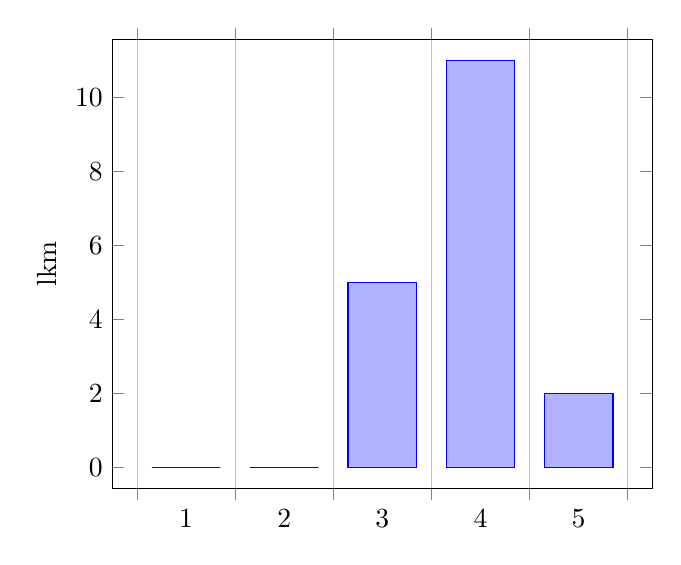
\begin{tikzpicture}
\begin{axis}[x tick label 
style={/pgf/number format/1000 sep=}, ylabel=lkm, enlargelimits=0.05, legend style={at={(0.5,-0.15)}, anchor=north,legend columns=-1},ybar interval=0.7]
\addplot coordinates {(1,0) (2,0) (3,5) (4,11) (5,2) (6,0)}; % miksei piirrä vikaa asiaa? :3
\end{axis}
\end{tikzpicture}
\caption{``Harjoituskurssista on ollut minulle hyötyä.''}
\end{figure}

\subsection{Kisälliopetus}
Kurssi toteuttaa kisälliopetuksen piirteet opiskelijoiden vastauksien mukaan hyvin.
Suurin osa opiskelijoista ($n=12$) kiitteli vastauksissaan sitä, että apua on saatavilla hyvin.
Loput ($n=7$) opiskelijat eivät kommentoineet vastausta, mutta olivat jokseenkin samaa mieltä tai täysin samaa mieltä siitä, että kurssilla saa apua hyvin.
Kysymyksen avoimeen perusteluosioon vastasi yheksän ($n=9$) opiskelijaa. Vastauksista kävi ilmi, että opiskelijat kokivat, että harjoituskurssilla saa paremmin apua tehtävien tekoon kuin tavallisella kurssilla, sillä ryhmä on pienempi, kaikki aika käytetään laskemiseen ja että paikalla on auskuja. Avun saamista tehtävien ratkaisemisessa kiiteltiin kurssin parhaimpana puolena: ``Suurin plussa! että saa pua''. 

Avoimeen kysymykseen ``Saatko sellaista apua, mitä kaipaat? Minkälaista apua kaipaat matematiikassa?'' kolmetoista ($n=13$) vastasi myöntävästi sekä kaipaavansa apua ja yksi vastasi, ettei kaipaa apua. Neljä opiskelijaa jätti vastaamatta kysymykseen. 

Myönteisissä vastauksissa esimerkiksi kaivattiin jotakuta selventämään kysymystä: ``Välillä on vaikea hahmottaa, mitä kysymys minulta haluaa joten opettajan läsnäolo ja tarvittaessa apu on helpottanut vaikeimpien tehtävien tekoa merkittävästi.'' , ``Kyllä lisää selitystä kaivataan''. Vaikeissa ja soveltavissa tehtävissä kaivattiin apua: ``Kyllä, tarvitsen apua joihinkin vaikeisiin tehtäviin'', Saan hyvin apua. Usein kaipaa apua vaikeimpiin sovelluksiin.''. 

Opettajan osuutta kiiteltiin, erityisesti sitä, että opettaja osaa neuvoa silloinkin, kun ei itsekään tiedä mitä kysyisi: ``Yleensä en osaa sanoa millaista apua kaipaan, mutta Päivi osaa aina neuvoa :)''. Myös laskimen käytössä kaivattiin ja oli saatu apua kurssilla. 

\begin{figure}[h!]
\centering
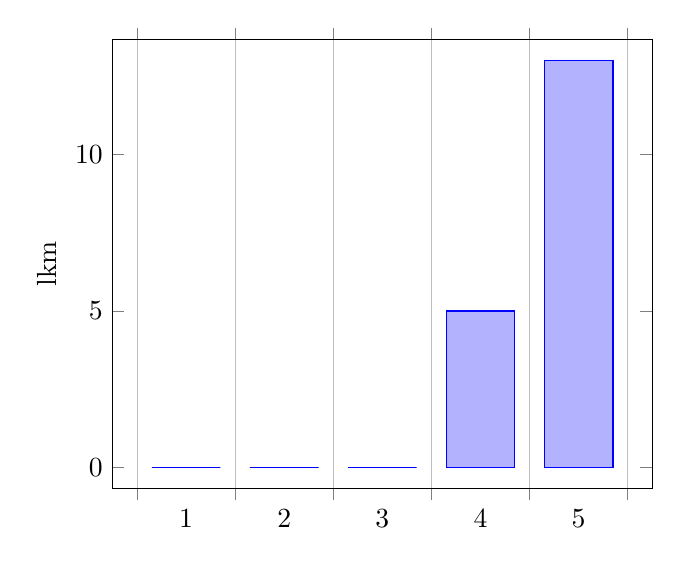
\begin{tikzpicture}
\begin{axis}[x tick label 
style={/pgf/number format/1000 sep=}, ylabel=lkm, enlargelimits=0.05, legend style={at={(0.5,-0.15)}, anchor=north,legend columns=-1},ybar interval=0.7]
\addplot coordinates {(1,0) (2,0) (3,0) (4,5) (5,13) (6,0)}; % miksei piirrä vikaa asiaa? :3
\end{axis}
\end{tikzpicture}
\caption{``Saan harjoituskurssilla apua tehtävien ratkaisemiseen.''}
\end{figure}

Myös \emph{scaffolding}-ilmiö esiintyy vastauksissa.

\begin{figure}[h!]
\centering
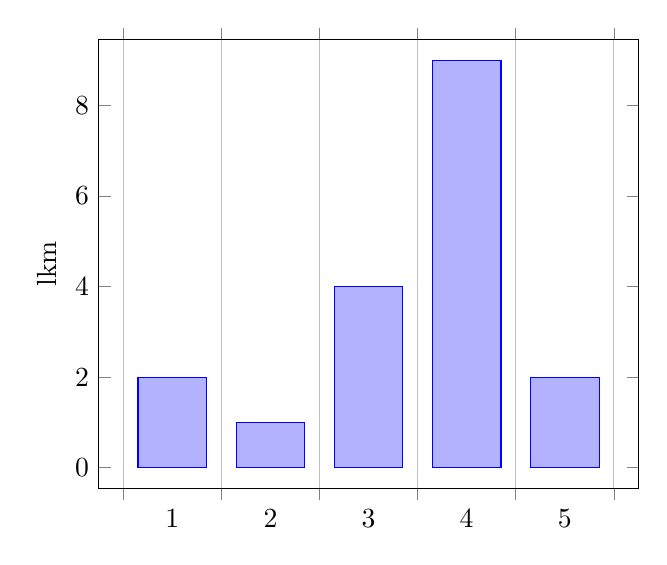
\begin{tikzpicture}
\begin{axis}[x tick label 
style={/pgf/number format/1000 sep=}, ylabel=lkm, enlargelimits=0.05, legend style={at={(0.5,-0.15)}, anchor=north,legend columns=-1},ybar interval=0.7]
\addplot coordinates {(1,2) (2,1) (3,4) (4,9) (5,2) (6,0)}; % miksei piirrä vikaa asiaa? :3
\end{axis}
\end{tikzpicture}
\caption{``Saan harjoituskurssilla tehtyä sellaisiakin tehtäviä, joita en itsenäisesti osaisi tehdä.''}
\end{figure}

Itsevarmuus omasta osaamisesta vaikuttaa opiskelijan matematiikkapelkoon.
Se, että opiskelija kokee korkeaa minäpystyvyyden tunnetta on myös välttämätöntä \emph{flow}-tilaan pääsemiseksi.
%Vastauksista voi myös päätellä, että harjoituskurssi torjuu opiskelijoiden matematiikkapelkoa.

\begin{figure}[h!]
\centering
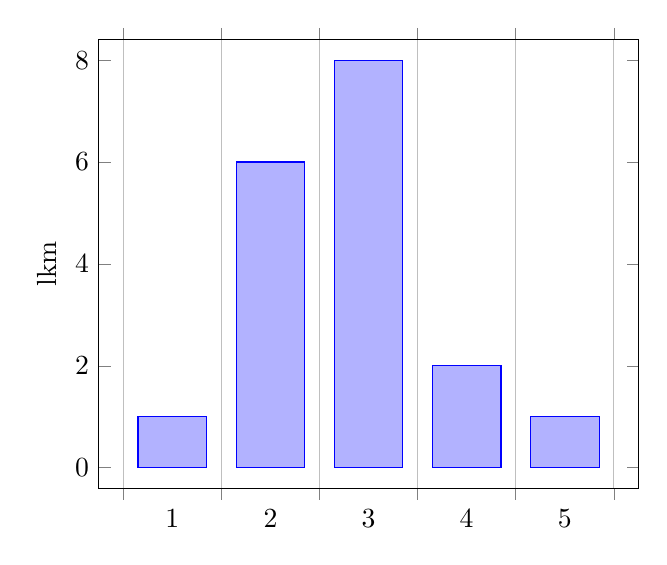
\begin{tikzpicture}
\begin{axis}[x tick label 
style={/pgf/number format/1000 sep=}, ylabel=lkm, enlargelimits=0.05, legend style={at={(0.5,-0.15)}, anchor=north,legend columns=-1},ybar interval=0.7]
\addplot coordinates {(1,1) (2,6) (3,8) (4,2) (5,1) (6,0)};
\end{axis}
\end{tikzpicture}
\caption{``Harjoituskurssi on lisännyt itsevarmuuttani matematiikan osaamisen suhteen.''}
\end{figure}

Opiskelijat, jotka olivat täysin tai jokseenkin eri mieltä väitteen kanssa vastasivat muun muassa, että itsevarmuus riippuu vain käsiteltävien aiheiden mielekkyydestä, että yksi kurssi ei riitä itsevarmuuden kehittämiseen ja että itsevarmuutta vähentää se, että ei saa helpoksi luonnehdittua tehtävää ratkaistua. 

On mielenkiintoista, että menestys matematiikan kursseilla ei välttämättä paranna itsetuntoa matematiikan osaamiseen suhteen. Vastauksista ilmeni esimerkiksi, että vaikka opiskelija koki harjoituskurssin parantaneen hänen menestystään muillakin matematiikan kursseilla, niin hän edelleen koki matematiikan vaikeaksi ja etenemistahdin liian nopeaksi. Yleisesti ottaen kuitenkin ne, joiden mielestä kurssi oli parantanut heidän menestystään, kokivat, että se oli myös lisännyt heidän itsevarmuuttaan, ja päin vastoin.

Opiskelijat, jotka oli samaa tai täysin samaa mieltä perustelivat vastaustaan esimerkiksi siten, että laskemisen määrän koettiin edistävän oppimista ja lisäävän itsetuntoa: ``Lasken enemmän ja saan apua -> edistyn'', ``Harjoitus tekee mestarin''. 



\subsection{Opiskelijoiden matematiikkakuva}
Kyselyvastauksista kävi ilmi, että moni opiskelija pitää matematiikkaa enimmäkseen laskemisena.
Lisäksi matemaattisen taidon koetaan kehittyvän harjoittelun avulla.

\subsection{Viihtyvyys kurssilla}
Opiskelijoiden mielestä harjoituskurssilla oli pääosin mukavaa. Ainoastaan kaksi opiskelijaa oli väitteen ``Harjoituskurssilla on mukavaa'' kanssa eri mieltä, ja perustelivat vastauksiaan kurssin tylsyydellä ja laskemisen puuduttavuudella. Yksi opiskelija ei ollut samaa eikä eri mieltä. Muut viisitoista ($n=15$) olivat joko samaa tai täysin samaa mieltä siitä, että kurssilla on mukavaa. Vastauksissa nousi positiivisena esille rento, ei-koulumainen ilmapiiri kurssilla, mahdollisuus jutella kavereiden kanssa, ratkoa tehtäviä yhdessä ja syödä laskemisen lomassa. Opiskelijat kokivat myös, että suhde opettajaan oli harjoituskurssilla välittömämpi. 

Toisaalta vapaus kurssilla koettiin myös ongelmaksi; eräs opiskelija reflektoi omaa panostaan kurssilla seuraavasti: ``Kurssilla on hyvä tunnelma ja vapaampaa puhua kavereiden kanssa. Tämä toisaalta on myös ongelma ja mietinkin joskus että puhua voisi vapaa-ajallakin ja että onko kurssi turha minulle''



\subsection{Kurssin vaativuustaso}
Osalle opiskelijoista kurssi oli sopivan vaativa, mutta monet kokivat myös tylsistyvänsä tunnilla.
Tämä tarjoaisi hedelmällisen mahdollisuuden eriyttää opetusta; jos tehtävämonisteita olisi kaksi, kertaava ja syventävä, kurssi palvelisi laajempaa opiskelijajoukkoa.
Koska kurssisuoritukseen riittää vain läsnäolo, valmistaa kurssi myös korkeakoulujen akateemiseen vapauteen; opiskelijalla on vastuu omasta työskentelystään.
Tämä saattaa lisäksi hillitä matematiikkapelkoa, sillä opiskelijalla ei ole paineita suorittaa tiettyä määrää tehtävistä.

\subsection{Miten kurssia voisi kehittää?}
Opiskelijoiden vastauksista ei noussut mitään yhtä erityistä kehitysideaa, vaan ideoita oli vaihtelevasti. Kahdeksan ($n=8$) opiskelijaa jätti vastaamatta kysymykseen ja kolme ($n=3$) vastasi ``en tiedä''. Lopuissa vastauksissa toivottiin jotkin muuta ajankohtaa kurssille, lisää opettajia tai ohjaajia, hauskempia ja pohtimista vaativia tehtäviä, opittujen asioiden syventämistä. Myös toivottiin, että tehtyjen tehtävien määrälle asetettaisiin jokin vähimmäisraja, jotta se motivoisi tekemään tehtäviä. Yksi opiskelija vastasi, että kurssi on ollut hyvä näin. 




\pagebreak
\section{Pohdintaa}


\subsection{Kehittämisehdotuksia}


\pagebreak

\printbibliography
\pagebreak
\begin{appendices}
\section{Kyselylomake}
Käyttämämme kyselylomake on seuraavilla sivuilla.
\end{appendices}

\end{document}
